\documentclass[10pt]{article}

%------------------------------------------------------
%   PACKAGES
%------------------------------------------------------

% Default 
\usepackage{graphicx}
\usepackage[backend=biber,
  style=numeric, 
  sorting=none]{biblatex}

% Additional
\usepackage{amsmath}
\usepackage{textcomp, gensymb}
\usepackage{placeins}
\usepackage{tabularray} 
\usepackage{xcolor}
\usepackage{placeins}
\usepackage{csquotes}
\usepackage{todonotes}

\newcommand{\td}[1]{\todo[linecolor=blue, backgroundcolor=blue!25,bordercolor=blue, size=\small, inline]{#1}}

\addbibresource{references.bib}

\title{Thin Lens} 
\author{Rahmanyaz Annyyev, Hikmat Gulaliyev}
\date{29 March 2024} 

\begin{document}

\maketitle

\begin{abstract}

\end{abstract}

\section{Introduction}

In the most general sense, a \textbf{lens} is a refracting body that redirects the light rays passing through it. It either focuses or diverges the light rays, depending on the shape of the lens. A simple lens consists of a single piece of transparent material, whereas a compound lens consists of several simple lenses, called \textit{elements}, usually arranged along a common axis. Lenses are usually made of glass or plastic and are comprised of two surfaces, one or both of which are curved. The main purpose of a lens is to form an image of an object. The image can be real or virtual, depending on the position of the object relative to the lens. A real image is formed when the light rays converge at a point, whereas a virtual image is formed when the light rays diverge from a point \cite{Giancoli_2014}. 

\begin{figure}[hbt!]
  \centering
  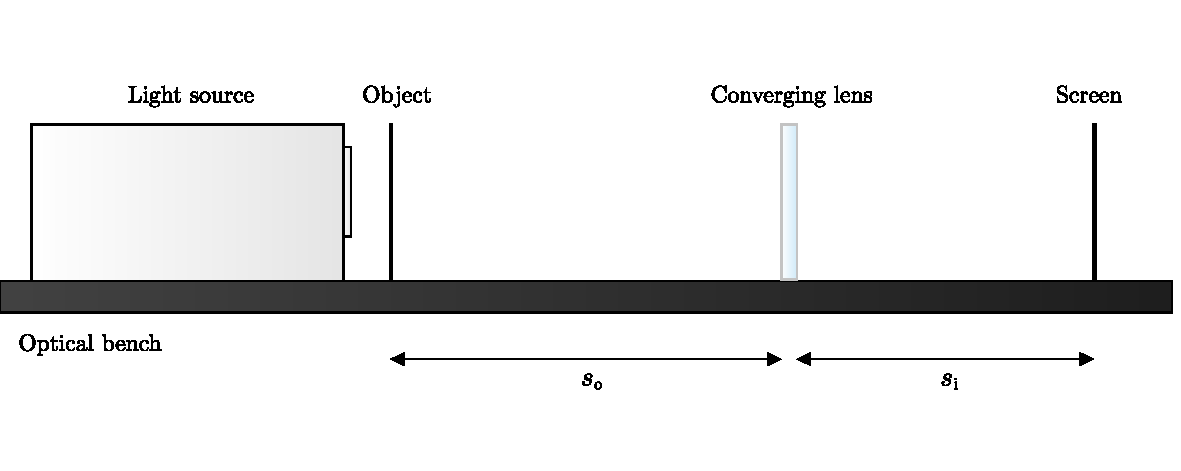
\includegraphics[scale=0.5]{figures/f1.pdf}
  \caption{The converging lens.}
  \label{fig:1}
\end{figure}

The most common types of lenses are \textbf{converging} (convex) and \textbf{diverging} (concave) lenses. A converging lens is thicker in the middle than at the edges and focuses light rays to a point called the focal point. A diverging lens is thinner in the middle than at the edges and spreads light rays apart. The focal length of a lens is the distance between the lens and the focal point. The focal length of a converging lens is positive, whereas the focal length of a diverging lens is negative. The \textbf{thin lens equation} relates the object distance, the image distance, and the focal length of a lens. The equation is given by
\begin{equation}
  \label{eq:1}
  \frac{1}{f} = \frac{1}{s_{\text{o}}} + \frac{1}{s_{\text{i}}},
\end{equation}
where $f$ is the focal length of the lens, $s_{\text{o}}$ is the object distance, and $s_{\text{i}}$ is the image distance \cite{Pedrotti_2006}.  

\begin{figure}[hbt!]
  \centering
  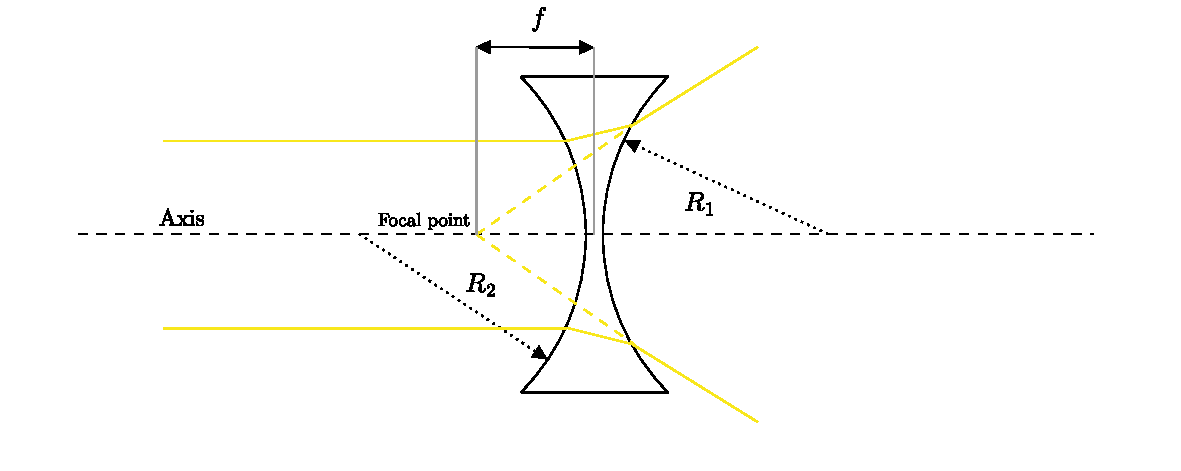
\includegraphics[scale=0.5]{figures/f2.pdf}
  \caption{The diverging lens.}
  \label{fig:2}
\end{figure}

Lenses are divided into two categories: thin lenses and thick lenses. A thin lens is a lens whose thickness is negligible compared to the radii of curvature of the lens surfaces. A thick lens is a lens whose thickness is not negligible compared to the radii of curvature of the lens surfaces. This division depends on a given problem and the accuracy required \cite{Hecht_2017}. 

The experiment consists of three parts: A, B, and C. The experimental setup is comprised of a $150$ mm converging lens, a $75$ mm diverging lens, a light source, a crossed arrow target that represents an object, and a screen on which the image is formed. The lenses will be assumed to be thin lenses.

\subsection*{Part A}

\begin{figure}[hbt!]
  \centering
  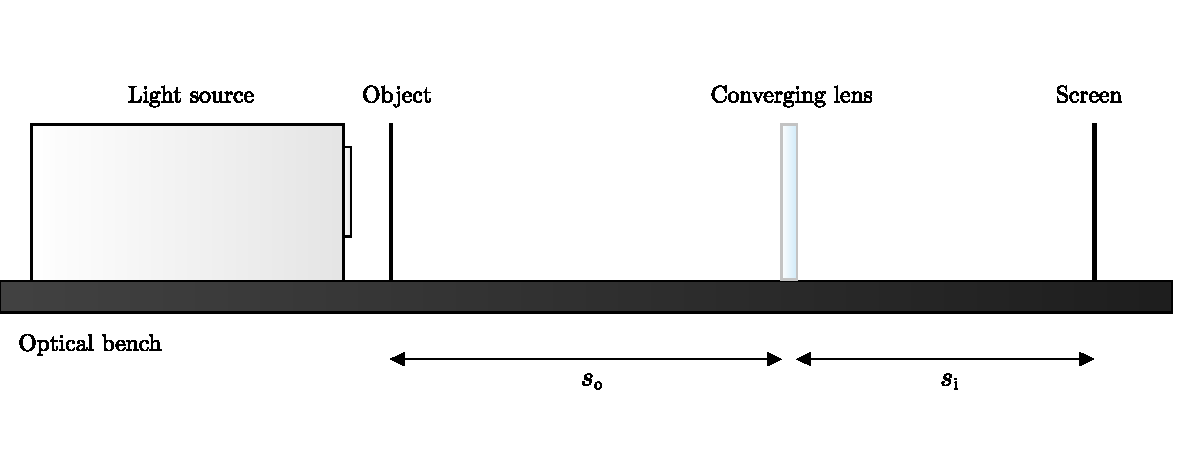
\includegraphics[scale=0.5]{figures/f3.pdf}
  \caption{The experimental setup of part A.}
  \label{fig:3}
\end{figure}

In part A, we will employ the thin lens equation to determine the focal length of the converging lens. The setup is shown in Figure~\ref{fig:3}. The thin lens equation is given in Equation~\ref{eq:1}. First, we place the converging lens on the optical bench and adjust its position to obtain a sharp image of the object on the screen. We measure the object distance, $s_{\text{o}}$, from the lens to the object's position and the image distance, $s_{\text{i}}$, from the lens to the screen's position. We repeat this process two more times with different object distances.

\subsection*{Part B}

\begin{figure}[hbt!]
  \centering
  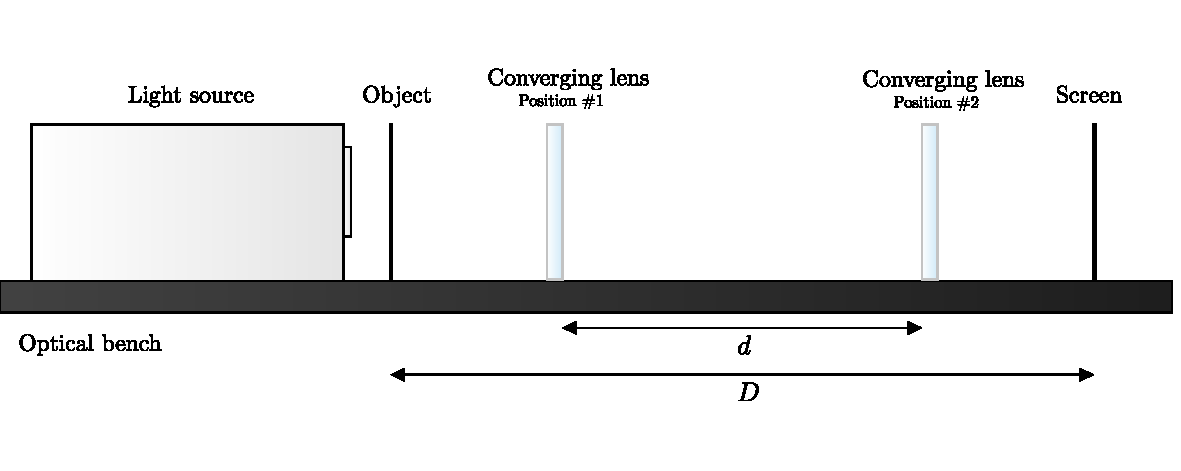
\includegraphics[scale=0.5]{figures/f4.pdf}
  \caption{The experimental setup of part B.}
  \label{fig:4}
\end{figure}

In part B, we will use the Bessel method to determine the focal length of the converging lens. The setup is shown in Figure~\ref{fig:4}. The formula used in the Bessel method is given by
\begin{equation}
  f = \dfrac{D^2 - d^2}{4D},
\end{equation}
where $f$ is the focal length of the lens, $D$ is the distance between the two positions of the screen, and $d$ is the distance between the two positions of the lens. First, we place the converging lens on the optical bench such that the object distance, $s_{\text{o}}$, is at least four times the estimated focal length of the lens. Next, we determine two positions of the lens that produce a sharp image of the object on the screen. We measure the distance between the two positions of the lens, $d$, and the distance between the two positions of the screen, $D$. We repeat this process two more times with different object distances.

\subsection*{Part C}

\begin{figure}[hbt!]
  \centering
  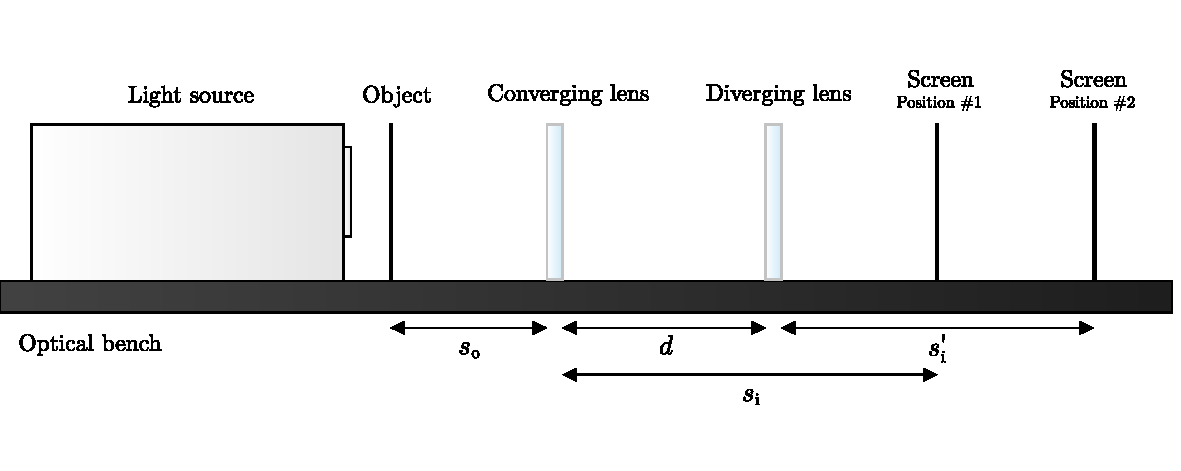
\includegraphics[scale=0.5]{figures/f5.pdf}
  \caption{The experimental setup of part C.}
  \label{fig:5}
\end{figure}

In part C, we will use the virtual object method to determine the focal length of the diverging lens. The setup is shown in Figure~\ref{fig:5}. It is not possible to directly measure the focal length of a diverging lens using the previous methods because the image formed by a diverging lens is always virtual. In the virtual object method, we use a converging lens to create a real image of the object, which then serves as a virtual object for the diverging lens. The converging lens should be sufficiently \enquote{strong} to satisfy the condition 
\begin{equation}
  \dfrac{1}{f_{\text{c}}} > \left| \dfrac{1}{f_{\text{d}}} \right|,
\end{equation}
where $f_{\text{c}}$ is the focal length of the converging lens and $f_{\text{d}}$ is the focal length of the diverging lens. If this condition is not satisfied, the image formed by the converging lens will be virtual, and the virtual object method will not work. The formula used in the virtual object method is given by
\begin{equation}
  f = \dfrac{s^{'}_{\text{i}} \left( s_{\text{i}} - d \right)}{s_{\text{i}} - \left( s^{'}_{\text{i}} + d \right)},
\end{equation}
where $f$ is the focal length of the diverging lens, $s_{\text{i}}$ is the distance between the first position of the screen and the converging lens, $s^{'}_{\text{i}}$ is the distance between the second position of the screen and the diverging lens, and $d$ is the distance between the lenses. First, we mount the converging lens on the optical bench such that the object distance, $s_{\text{o}}$, is in the range of $10$ to $12$ cm. Then, we adjust the position of the screen to obtain a sharp image of the object. We measure the image distance, $s_{\text{i}}$, from the lens to the screen's first position. Next, we place the diverging lens on the optical bench and adjust the screen to obtain a sharp image of the object. We measure the image distance, $s'_{\text{i}}$, from the lens to the screen's second position. We measure the distance between the two positions of the screen, $d$. We repeat this process two more times with different object distances.

\section{Discussion \& Conclusion}

\section{Data \& Results}

\subsection*{Part A}

The results of part A are shown in Table~\ref{tab:1}. 

\begin{table}[ht]
  \centering
  \vspace{4mm}
  \begin{tblr}{
    cells = {halign = c, valign = m},
    row{odd} = {bg = lightgray!5},
    row{1} = {bg = lightgray!20},
    hlines = {},
    vlines = {},
    cell{5}{2}={c=2}{c},
    cell{6}{2}={c=2}{c}
  }
    $s_{\text{o}}$ (cm) & $s_\text{{i}}$ (cm) & Focal length, $f_{\text{m}}$ (cm) \\
    \hline
    18 & 12.5 & 7.38 \\
    28 & 10.5 & 7.63 \\
    19.5 & 12.2 & 7.50 \\
    \hline
    Average focal length, $\bar{f}$ (cm) & Error, $\Delta \bar{f}$ (cm) & \\
    7.50 & 0.13 \\ 
  \end{tblr}
  \caption{Results of part A of the experiment.}
  \label{tab:1}
\end{table}

\subsection*{Part B}

The results of part B are shown in Table~\ref{tab:2}.

\begin{table}[ht]
  \centering
  \vspace{4mm}
  \begin{tblr}{
    cells = {halign = c, valign = m},
    row{odd} = {bg = lightgray!5},
    row{1} = {bg = lightgray!20},
    hlines = {},
    vlines = {},
    cell{5}{2}={c=2}{c},
    cell{6}{2}={c=2}{c}
  }
    $d$ (cm) & $D$ (cm) & Focal length, $f_{\text{m}}$ (cm) \\
    \hline
    20.5 & 39.7 & 7.28 \\
    24.5 & 43 & 7.26 \\
    11.2 & 33 & 7.30 \\
    \hline
    Average focal length, $\bar{f}$ (cm) & Error, $\Delta \bar{f}$ (cm) & \\
    7.28 & 0.02 \\ 
  \end{tblr}
  \caption{Results of part B of the experiment.}
  \label{tab:2}
\end{table}

\subsection*{Part C}

The results of part C are shown in Table~\ref{tab:3}. The average focal length of the diverging lens is $-15.1$ cm with an error of $0.95$ cm. It is within the limits of error of the actual focal length of the lens, which is $-15$ cm.

\begin{table}[ht]
  \centering
  \vspace{4mm}
  \begin{tblr}{
    cells = {halign = c, valign = m},
    row{odd} = {bg = lightgray!5},
    row{1} = {bg = lightgray!20},
    hlines = {},
    vlines = {},
    cell{5}{2}={c=3}{c},
    cell{6}{2}={c=3}{c}
  }
    $s_{\text{i}}$ (cm) & $s'_{\text{i}}$ (cm) & d (cm) & Focal length, $f_{\text{m}}$ (cm) \\
    \hline
    16.4 & 22.8 & 7 & -16.0 \\
    18 & 25 & 9 & -14.1 \\
    21 & 46 & 9.6 & -15.2 \\
    \hline
    Average focal length, $\bar{f}$ (cm) & Error, $\Delta \bar{f}$ (cm) & \\
    -15.1 & 0.95 \\ 
  \end{tblr}
  \caption{Results of part C of the experiment.}
  \label{tab:3}
\end{table}

\section{Extra credit}

\td{Write a comprehensive essay on the applications of lenses in various fields. Use at least two references because I believe we will not be granted any extra credit points if we do not use references. Please don't use non-scientific sources.}

Lenses are a ubiquitous part of our daily lives. They are used in cameras, microscopes, telescopes, and many other devices. In this experiment, we have learned how to determine the focal length of a lens using the thin lens equation, the Bessel method, and the virtual object method. We have also learned how to calculate the magnification of a lens.

\printbibliography

\end{document}